\documentclass[a4paper]{article}

\usepackage[utf8]{inputenc}
\usepackage[T1]{fontenc}
\usepackage{textcomp}
\usepackage{amsmath, amssymb}
\usepackage{array,multirow,graphicx}
\usepackage{booktabs}
\usepackage{hyperref}
\usepackage{subcaption}
\usepackage{biblatex}
\addbibresource{report.bib}


% figure support
\usepackage{import}
\usepackage{xifthen}
\pdfminorversion=7
\usepackage{pdfpages}
\usepackage{transparent}
\newcommand{\incfig}[1]{%
	\def\svgwidth{\columnwidth}
	\import{./figures/}{#1.pdf_tex}
}

\pdfsuppresswarningpagegroup=1


\title{NPFL103 Information Retrieval: Assignment 1}
\date{\today}
\author{Andrew McIsaac}

\begin{document}
\maketitle

\section{Introduction}
This report examines using the vector-space model for information retrieval on
sets of documents in both English and Czech. I explore different ways to create
an inverted index for both languages, examining which techniques work best for
the two different languages, and further go on to examine different techniques
for improving results, including modifying weightings of terms and documents,
and different approaches towards document length normalization. The results
for a baseline system (run-0) and an improved system (run-1) are shown and
discussed.

\section{Preprocessing and Index Construction}
To create the inverted index, I first processed the documents by creating
intermediate files consisting of (term, docID) pairs for every term in every
document, as well as equivalent (docID, [terms]) pairs, consisting of document
id and the list of terms in the document. The terms were extracted from the xml
structure. From the Czech documents, I kept terms that were tagged with
Geography, Title, Heading, and Text. From the English documents, I kept terms
that were tagged with PH, KH, HD, DH, SE, DL, LD, TE, CP, DC, CR, DP, and SM.

For the baseline system these terms were left in their word forms. In the
improved version, I removed stopwords (using a list of stopwords from the
\texttt{spacy} and \texttt{spacy\_udpipe} python packages for English and Czech
respectively), performed case-folding and experimented with both lemmatization
and stemming of queries and documents. Lemmatization used the \texttt{spacy} and
\texttt{spacy\_udpipe} packages for the respective languages, while for English
stemming the \texttt{nltk} package was used with the \texttt{PorterStemmer}.
\texttt{nltk} does not have Czech stemming capabilities, so the documents and
queries were stemmed with this 
\href{https://github.com/UFAL-DSG/alex/blob/master/alex/utils/czech_stemmer.py}
{Czech Stemmer} implementation based on the SnowballStemmer. Experimentation
results for the various preprocessing methods are discussed in Section
\ref{sec:preproc}.

With the processed documents, I use the single-pass in-memory indexing (SPIMI)
algorithm to create an inverted index for each file. These files are then merged
together to create the final inverted index, and this is saved on disk.

\section{Query Processing and Retrieval}
With the list of topics, I created a dictionary of \texttt{topic\_num:[terms]}
for all topics, where the terms are the tokenized and processed terms from the
title of each topic, preprocessed in the same way as the document terms for each
experiment. For the baseline model, I then proceed to compute the cosine
similarity between the query terms and documents for each topic, using the
\texttt{FastCosineScore} algorithm from Manning et al. \cite[p.~125]{iir}. A
heap is then used to retrieve the top 1000 documents for the query, which is
sorted by score and saved for evaluation.

\section{Baseline Results}
With the constrained baseline results as specified in the assignment brief, my
system achieved a mean average precision (MAP) score of 0.0597 on the Czech
training topics, and a P$_{10}$ score of 0.0840. The averaged 11-point
precision/recall graph is shown in Fig. \ref{fig:cs_train}.

For the English documents, the baseline MAP score was 0.0445, with a P$_{10}$
score of 0.0840. The averaged 11-point precision/recall graph is shown in Fig.
\ref{fig:en_train}.

\begin{figure}[htpb]
	\centering
	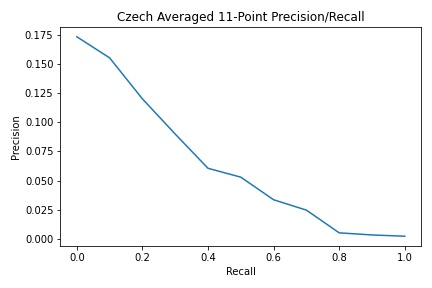
\includegraphics[width=0.8\textwidth]{plot_run-0_cs_precision_recall.jpg}
	\caption{Averaged 11-point Precision/Recall for Czech training data on run-0}
	\label{fig:cs_train}
\end{figure}

\begin{figure}[htpb]
	\centering
	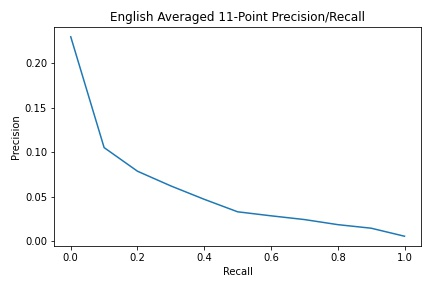
\includegraphics[width=0.8\textwidth]{plot_run-0_en_precision_recall.jpg}
	\caption{Averaged 11-point Precision/Recall for English training data on run-0}
	\label{fig:en_train}
\end{figure}

\section{Experiments}

\subsection{Preprocessing Methods for Indexing}
\label{sec:preproc}
I experimented with stopwords, lemmatization and stemming. In every case, I also
converted all words to lower case. The results are shown in Table
\ref{tab:terms}. 

\begin{table}[htpb]
	\centering
	\caption{Mean average precision (MAP) and $P_{10}$ precision of the first 10
		documents training performance with different preprocessing techniques.\\
	wf: word forms, sw: stopwords, l: lemmatization, s: stemming\\}
	\label{tab:terms}
	\begin{tabular}{@{}l|ccccc@{}}
		\toprule
		Language & & wf & sw & sw+l & sw+s \\
		\cmidrule(r){1-1}\cmidrule(lr){2-2}\cmidrule(lr){3-3}\cmidrule(lr){4-4}\cmidrule(lr){5-5}\cmidrule(l){6-6}
		English & MAP & 0.0445 & 0.1244 & 0.0834 & \textbf{0.1751} \\
				& \small{$P_{10}$} & \small{0.084} & \small{0.172} & \small{0.136} & \small{0.252} \\
		\cmidrule(r){1-1}\cmidrule(lr){2-2}\cmidrule(lr){3-3}\cmidrule(lr){4-4}\cmidrule(lr){5-5}\cmidrule(l){6-6}
		Czech & MAP & 0.0597 & 0.0770 & \textbf{0.1553} & 0.0672 \\
			  & \small{$P_{10}$} & \small{0.084} & \small{0.100} & \small{0.148} & \small{0.060} \\
		\bottomrule
	\end{tabular}
\end{table}

For English documents, preprocessing with stopwords lists and stemming produced
the best results, both for MAP and $P_{10}$, while using stopwords lists and
lemmas produced the best results for Czech documents.

\subsection{Term/Document Frequency Weighting}
I experimented with different term frequency and document frequency weighting
scores. From Table \ref{tab:tfidf} it can be seen that for both languages there
is significant performance improvement on the training data with natural term
frequency weighting, and either inverse document frequency or probabilistic idf
for both English and Czech documents, with prob idf marginally better than 
standard idf in both cases. Using a different term weighting than just term
frequency (logarithm or augmented) produced significantly weaker results.

\begin{table}[htpb]
	\centering
	\caption{Mean average precision (MAP) and $P_{10}$ precision of the first
		10 documents training performance with different tf-idf weightings.\\
	SMART notation tags are applied to both query and document in all cases.\\}
	\label{tab:tfidf}
	\begin{tabular}{@{}l|cccccc@{}}
		\toprule
		Language & & nnc & ntc & npc & ltc & apc \\
		\cmidrule(r){1-1}\cmidrule(lr){2-2}\cmidrule(lr){3-3}\cmidrule(lr){4-4}\cmidrule(lr){5-5}\cmidrule(lr){6-6}\cmidrule(l){7-7}
		English & MAP & 0.1751 & 0.2244 & \textbf{0.2248} & 0.1320 & 0.0469 \\
				& \small{$P_{10}$} & \small{0.252} & \small{0.328} & \small{0.328} & \small{0.172} & \small{0.092} \\
		\cmidrule(r){1-1}\cmidrule(lr){2-2}\cmidrule(lr){3-3}\cmidrule(lr){4-4}\cmidrule(lr){5-5}\cmidrule(lr){6-6}\cmidrule(l){7-7}
		Czech & MAP & 0.1553 & 0.1933 & \textbf{0.1947} & 0.0879 & 0.0922 \\
		& \small{$P_{10}$} & \small{0.148} & \small{0.224} & \small{0.228} & \small{0.096} & \small{0.100} \\
		\bottomrule
	\end{tabular}
\end{table}

\subsection{Pivoted document length normalization}

I experimented with using pivoted document length normalization instead of
cosine similarity. The pivot value was selected following the process described
in Singhal et al. \cite{singhal}. Fig. \ref{fig:cosine} shows document lengths
for retrieval and relevance with respect to their probabilities. With the
crossover point $p$ at document length $l_p$, the pivot value was determined as
the mean of the cosine normalization values for documents of length $l_p$. For
Czech, this was 24.6788, and for English this was 40.7795. 

\begin{figure}[htpb]
	\centering
	\begin{subfigure}{0.45\textwidth}
		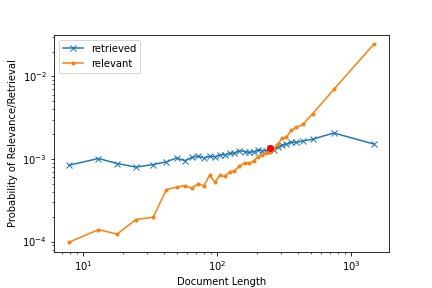
\includegraphics[width=\textwidth]{plot_cs_rel_ret.jpg}
		\caption{Czech}
		\label{fig:cs_cosine}
	\end{subfigure}
	\hfill
	\begin{subfigure}{0.45\textwidth}
		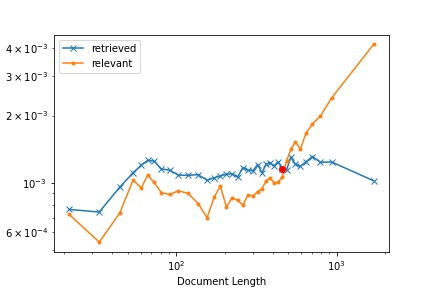
\includegraphics[width=\textwidth]{plot_en_rel_ret.jpg}
		\caption{English}
		\label{fig:en_cosine}
	\end{subfigure}
	\caption{Document lengths for retrieval using cosine normalization compared
	to relevance. The orange lines show the document lengths of relevant documents
	with respect to the probability of relevance, while the blue lines show the
	same for retrieved documents. The red circle indicates the crossover point
	in document length.}
	\label{fig:cosine}
\end{figure}

Table \ref{tab:pivot} shows MAP scores for different values of the scaling
factor $a$. The $P_{10}$ value for English with a scaling factor of 0.85 was
0.352. The $P_{10}$ value for Czech with a scaling factor of 0.9 was 0.232.

\begin{table}[htpb]
	\centering
	\caption{MAP training performance of pivoted document length normalization 
	with different values of scaling factor $a$\\}
	\label{tab:pivot}
	\begin{tabular}{@{}lcccccccc@{}}
		\toprule
		& 0.6 & 0.7 & 0.8 & 0.85 & 0.9 & 0.95 & cosine \\
		\cmidrule(r){1-1}\cmidrule(lr){2-2}\cmidrule(lr){3-3}\cmidrule(lr){4-4}\cmidrule(lr){5-5}\cmidrule(lr){6-6}\cmidrule(lr){7-7}\cmidrule(l){8-8}
		English & 0.2428 & 0.2442 & 0.2446 & \textbf{0.2453} & 0.2450 & 0.2423 & 0.2248 \\
		\cmidrule(r){1-1}\cmidrule(lr){2-2}\cmidrule(lr){3-3}\cmidrule(lr){4-4}\cmidrule(lr){5-5}\cmidrule(lr){6-6}\cmidrule(lr){7-7}\cmidrule(l){8-8}
		Czech & 0.1830 & 0.1869 & 0.1932 & 0.1938 & \textbf{0.2053} & 0.2010 & 0.1947 \\
		\bottomrule
	\end{tabular}
\end{table}

Fig. \ref{fig:pivot} shows how the lengths of the retrieved documents was
affected by pivoted document length normalization, with a closer correlation to
relevance for both Czech and English compared to retrieval using cosine
normalization. But while the close line for English, particularly for small to
medium length documents corresponded with the best MAP score on the training
data, the value of the scaling factor $a=0.6$ which produced very similar document
lengths for retrieval and relevance for the Czech documents performed worse
than $a=0.9$, with a MAP of 0.1830 compared to 0.2053.

\begin{figure}[htpb]
	\centering
	\begin{subfigure}{0.3\textwidth}
		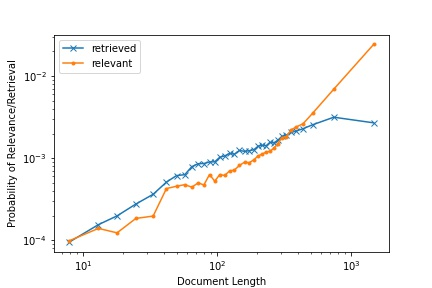
\includegraphics[width=\textwidth]{plot_cs_rel_ret_pivoted0_6.jpg}
		\caption{Czech, $a = 0.6$}
		\label{fig:cs_pivot}
	\end{subfigure}
	\hfill
	\begin{subfigure}{0.3\textwidth}
		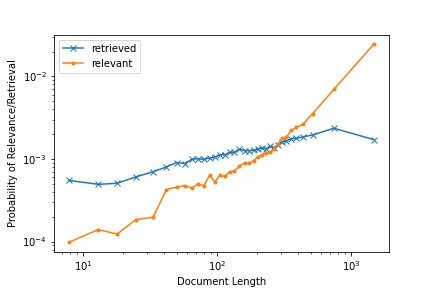
\includegraphics[width=\textwidth]{plot_cs_rel_ret_pivoted0_9.jpg}
		\caption{Czech, $a = 0.9$}
		\label{fig:cs_pivot}
	\end{subfigure}
	\hfill
	\begin{subfigure}{0.3\textwidth}
		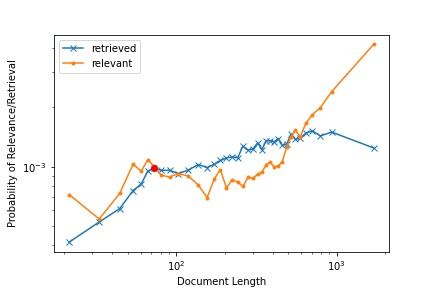
\includegraphics[width=\textwidth]{plot_en_rel_ret_pivoted.jpg}
		\caption{English, $a = 0.85$}
		\label{fig:en_pivot}
	\end{subfigure}
	\caption{Document lengths for retrieval using pivoted document length
	normalization compared to relevance.}
	\label{fig:pivot}
\end{figure}

\section{Run-1 Results}

The best Czech system achieved a mean average precision score of 0.2053, with a
$P_{10}$ score of 0.232. This was obtained by preprocessing the documents and
queries by filtering stopwords and lower-casing and lemmatizing words. Natural
term weighting and probabilistic idf document weighting achieved the best
performance in my experiments, so this was used, and pivoted document length
normalization was also used with a scaling factor of 0.9. The precision/recall
graph for the Czech training topics is shown in Fig. \ref{fig:cs_train_run_1}.

The best system for English achieved a mean average precision score of 0.2453,
and a $P_{10}$ score of 0.352. The parameters for achieving this were that the
documents were preprocessed by filtering stopwords, lower-casing, and stemming
every word. Further, natural term weighting and probabilistic idf document
weighting was used, and pivoted document length normalization was also used
with a scaling factor of 0.85. The precision/recall graph is shown in Fig.
\ref{fig:en_train_run_1}.

\begin{figure}[htpb]
	\centering
	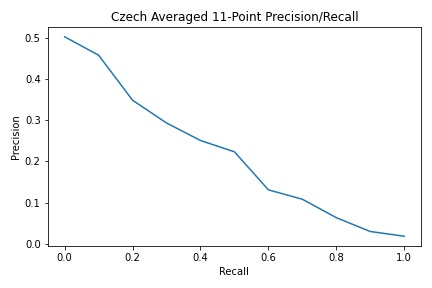
\includegraphics[width=0.8\textwidth]{plot_run-1_cs_precision_recall.jpg}
	\caption{Averaged 11-point Precision/Recall for Czech training data on run-1}
	\label{fig:cs_train_run_1}
\end{figure}

\begin{figure}[htpb]
	\centering
	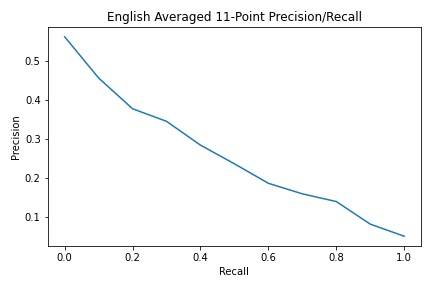
\includegraphics[width=0.8\textwidth]{plot_run-1_en_precision_recall.jpg}
	\caption{Averaged 11-point Precision/Recall for English training data on run-1}
	\label{fig:en_train_run_1}
\end{figure}

\section{Conclusion}
There was a significant performance increase from the baseline system to the
improved system (run-1). The largest performance increase for both languages
came from better preprocessing techniques, with the best improvement for English
yielding a +393\% MAP performance increase, while for Czech there was a +260\%
increase.

Better document weighting also led to substantial improvements, with
probabilistic inverse document frequency seen to be the best performing
technique for both languages on the training topics. Further, improving
document length normalization by using a pivot led to small improvements in both
languages, although for Czech it was not the case that the most precise mapping
of relevance and retrieval led to the highest performance increase.

The overall performance increase from the baseline system to the improved
system for English was +551\% MAP, +419\% $P_{10}$. For Czech the performance
increase was +343\% MAP, +276\% $P_{10}$.

Generally the approach for Czech and English was similar, although it differed
in some key areas. For Czech, lemmatization was found to work better, whereas
stemming worked much better for English. A possible reason for this is due to
the morphological richness of Czech compared to English, which means that
stemming maybe misses some inflections of Czech that it wouldn't for English.
It is also possible that the stemmer for Czech was missing some rules, or that
it was overly aggressive and lost a lot of precision on certain terms where
precise terms were stemmed and the effective meaning of the term was altered.
Also, the best scaling factor for pivoted document length normalization was
slightly different for Czech compared to English, although this was marginal.

\printbibliography

\newpage

\appendix

\section{Set Up and Running Experiments}

Make sure all requirements are installed:
\begin{verbatim}
pip install -r requirements.txt
python -c "import spacy_udpipe; spacy_udpipe.download('cs')"
python -m spacy download en_core_web_sm
\end{verbatim}

To run experiments run the following commands, replacing \texttt{train} with
\texttt{test} where appropriate to obtain results for the test topics.
The program must be run from the parent directory of the documents.
\begin{verbatim}
python run.py -q topics-train_en.xml -d documents_en.lst -r run-0_en
    -o run-0_train_en.res

python run.py -q topics-train_cs.xml -d documents_cs.lst -r run-0_cs
    -o run-0_train_cs.res

python run.py -q topics-train_en.xml -d documents_en.lst -r run-1_en 
    -o run-1_train_en.res --stopwords --lowercase --stemming
    --df-weighting prob_idf --pivoted 0.85

python run.py -q topics-train_cs.xml -d documents_cs.lst -r run-1_cs
    -o run-1_train_cs.res --stopwords --lowercase --lemmas
    --df-weighting prob_idf --pivoted 0.9
\end{verbatim}

The program will create an inverted index or load a saved one based on the value
of the -r parameter.  That is, if the same run parameter has been called before,
there will be a saved index which does not need to be recreated, and the queries
can be run directly on that. Otherwise, it will construct a new one before
running the queries.

\end{document}
